%!TEX root = ../report.tex

The following sections will outline the design steps taken to determine the force feedback characteristics.

\section{Force literature and Testing} % (fold)
\label{sec:force_literature_and_testing}

During the first client meeting, it was decided that the haptic feedback should apply 20 noticeable force increments from the joystick's top-dead position to the boundary of its range of motion. Conducting a literature review on the characteristics of human touch, it was discovered that the finger can detect a force as small as \SI{0.06}{\newton}, and only notices force changes which are 7\% or greater.
These values were used to form the hypothesis for the preliminary haptic tests (See Progress report).
The results of these tests showed that on average, the minimum force the users could detect is \SI{0.11}{\newton}, with a minimum noticeable increment of 10\%.
Additionally, two qualitative tests were conducted to find the maximum force a user could comfortably resist, and the ideal range of motion for various joystick lengths. The results showed that on average, the maximum force is \SI{1.19}{\newton} and the range of motion is \SI{90}{\degree} (\SIrange{-45}{45}{\degree}).

[Insert schematic here]

However, a range of 40 steps over \SI{90}{\degree} meant each increment would be \SI{2.25}{\degree}, and given encoder choice (see section X) with a precision of \SI{0.1}{\degree} this level of precision could not be achieved. It was therefore decided to increase this range to \SI{100}{\degree}, resulting in \SI{2.5}{\degree} steps which the encoders can accurately measure.

% section force_literature_and_testing (end)

\section{Step Design} % (fold)
\label{sec:step_design}

Using the maximum force range and increments specified in section X, namely 20 steps over \SIrange{0.11}{1.19}{\newton}, the actual relationship between force and joystick position could be established.

\begin{figure}
  % This file was created by matlab2tikz.
%
%The latest updates can be retrieved from
%  http://www.mathworks.com/matlabcentral/fileexchange/22022-matlab2tikz-matlab2tikz
%where you can also make suggestions and rate matlab2tikz.
%
\definecolor{mycolor1}{rgb}{0.00000,0.44700,0.74100}%

\tikzsetnextfilename{linear_force_location}
\centering
\begin{tikzpicture}
\begin{axis}[
  width=6.127in,
  height=4.279in,
  at={(1.028in,0.578in)},
  scale only axis,
  xmin=-50,
  xmax=50,
  xlabel style={font=\color{white!15!black}},
  xlabel={Shaft position ($^\circ$)},
  ymin=0,
  ymax=1.2,
  ylabel style={font=\color{white!15!black}},
  ylabel={Force (N)},
  axis background/.style={fill=white},
  title style={font=\bfseries},
  title={Linear force - location relationship},
]
\addplot [color=mycolor1, line width=1.5pt, forget plot]
  table[row sep=crcr]{%
-50	1.19\\
0	0.109999999999999\\
50	1.19\\
};
\end{axis}
\end{tikzpicture}%
  \caption{Linear force location relationship}
  \label{fig:linear_force_location}
\end{figure}

For a linear relationship, the force applied on the surgeon's finger would increase by \SI{0.054}{\newton} every \SI{2.5}{\degree} over the \SIrange{0.11}{1.19}{\newton} range, as shown in Figure~\ref{fig:linear_force_location}.

\begin{figure}
  % This file was created by matlab2tikz.
%
%The latest updates can be retrieved from
%  http://www.mathworks.com/matlabcentral/fileexchange/22022-matlab2tikz-matlab2tikz
%where you can also make suggestions and rate matlab2tikz.
%
\definecolor{mycolor1}{rgb}{0.00000,0.44700,0.74100}%
%
\centering
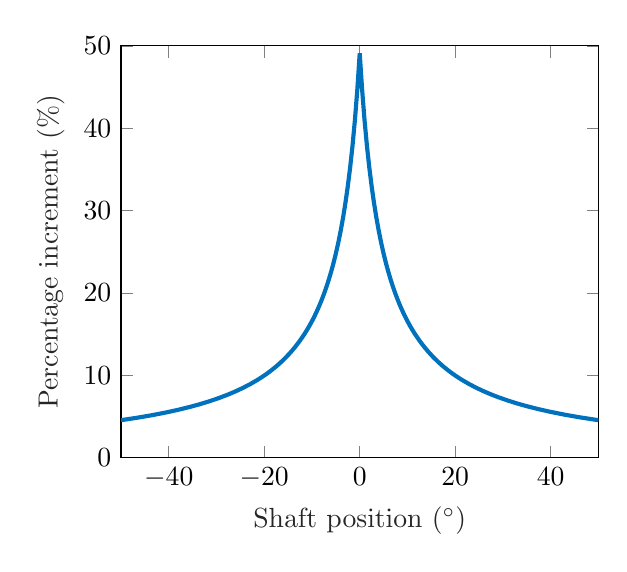
\begin{tikzpicture}
\begin{axis}[%
width=0.5\textwidth,
% width=4.472in,
% height=3.523in,
at={(0.75in,0.476in)},
scale only axis,
xmin=-50,
xmax=50,
xlabel style={font=\color{white!15!black}},
xlabel={Shaft position ($^\circ$)},
ymin=0,
ymax=50,
ylabel style={font=\color{white!15!black}},
ylabel={Percentage increment (\%)},
axis background/.style={fill=white},
% title style={font=\bfseries},
% title={Percentage increment per step for linear relationship},
% xmajorgrids,
% ymajorgrids
]
\addplot [color=mycolor1, line width=1.5pt, forget plot]
  table[row sep=crcr]{%
-50	4.53781512605042\\
-46.5	4.84565685570711\\
-43.5	5.14481707317074\\
-40.5	5.48334687246141\\
-38	5.80146110872368\\
-35.5	6.1587591240876\\
-33.5	6.47792706333973\\
-31.5	6.83198380566802\\
-29.5	7.22698072805139\\
-27.5	7.67045454545455\\
-26	8.04050029779631\\
-24.5	8.44806007509387\\
-23	8.89914304548451\\
-21.5	9.40111420612813\\
-20.5	9.7684515195369\\
-19.5	10.1656626506024\\
-18.5	10.596546310832\\
-17.5	11.0655737704918\\
-16.5	11.5780445969125\\
-15.5	12.1402877697842\\
-14.5	12.7599243856333\\
-13.5	13.4462151394422\\
-12.5	14.2105263157895\\
-11.5	15.0669642857143\\
-11	15.5350978135788\\
-10.5	16.0332541567696\\
-10	16.5644171779141\\
-9.5	17.1319796954315\\
-9	17.7398160315375\\
-8.5	18.3923705722071\\
-8	19.0947666195191\\
-7.5	19.8529411764706\\
-7	20.6738131699847\\
-6.5	21.5654952076677\\
-6	22.5375626043406\\
-5.5	23.6013986013986\\
-5	24.7706422018349\\
-4.5	26.0617760617761\\
-4	27.4949083503055\\
-3.5	29.0948275862069\\
-3	30.8924485125858\\
-2.5	32.9268292682927\\
-2	35.2480417754569\\
-1.5	37.9213483146067\\
-1	41.0334346504559\\
-0.5	44.7019867549669\\
0	49.0909090909091\\
0.5	44.7019867549669\\
1	41.0334346504559\\
1.5	37.9213483146067\\
2	35.2480417754569\\
2.5	32.9268292682927\\
3	30.8924485125858\\
3.5	29.0948275862069\\
4	27.4949083503055\\
4.5	26.0617760617761\\
5	24.7706422018349\\
5.5	23.6013986013986\\
6	22.5375626043406\\
6.5	21.5654952076677\\
7	20.6738131699847\\
7.5	19.8529411764706\\
8	19.0947666195191\\
8.5	18.3923705722071\\
9	17.7398160315375\\
9.5	17.1319796954315\\
10	16.5644171779141\\
10.5	16.0332541567696\\
11	15.5350978135788\\
11.5	15.0669642857143\\
12.5	14.2105263157895\\
13.5	13.4462151394422\\
14.5	12.7599243856333\\
15.5	12.1402877697842\\
16.5	11.5780445969125\\
17.5	11.0655737704918\\
18.5	10.596546310832\\
19.5	10.1656626506024\\
20.5	9.7684515195369\\
21.5	9.40111420612813\\
23	8.89914304548451\\
24.5	8.44806007509387\\
26	8.04050029779631\\
27.5	7.67045454545455\\
29	7.33297121129821\\
31	6.92662904053361\\
33	6.56295576081673\\
35	6.23556581986143\\
37.5	5.8695652173913\\
40	5.5441478439425\\
43	5.1983057373893\\
46	4.89307720188474\\
49.5	4.57937584803256\\
50	4.53781512605042\\
};
\end{axis}
\end{tikzpicture}%
  \caption{Percentage increment per step for linear relationship}
  \label{fig:percentage_increment_linear}
\end{figure}

However, from the surgeon's point of view, it feels like each step is getting smaller, as can be seen in Figure~\ref{fig:percentage_increment_linear}.
This shows that initially the surgeon detects large increments, but each individual force step after \SI{20}{\degree} will not be noticeable.
Thus, a logarithmic relationship between the force and the location was designed.

Solving equation~\ref{eq:logarithmic_increments} for the force values given,
\\
\begin{equation}
  F_{\text{min}} \times i^{20} = F_{\text{max}}
  \label{eq:logarithmic_increments}
\end{equation}

the increment ($i$) is 1.126, i.e. a 12.6\% increase for every \SI{2.5}{\degree}.
This is 2.6\% higher than the minimum found during testing.

The final force-position relationship is shown in equation~\ref{eq:final_force_pos}, and represented graphically in Figure~\ref{fig:logarithmic_force_location}.
\\
\begin{equation}
  F = 0.11 \times 1.126^{\frac{\theta}{2.5}}
  \label{eq:final_force_pos}
\end{equation}

Where $\theta$ is the angular position of the joystick.

\begin{figure}[hb]
  % This file was created by matlab2tikz.
%
%The latest updates can be retrieved from
%  http://www.mathworks.com/matlabcentral/fileexchange/22022-matlab2tikz-matlab2tikz
%where you can also make suggestions and rate matlab2tikz.
%
\definecolor{mycolor1}{rgb}{0.00000,0.44700,0.74100}%
\centering
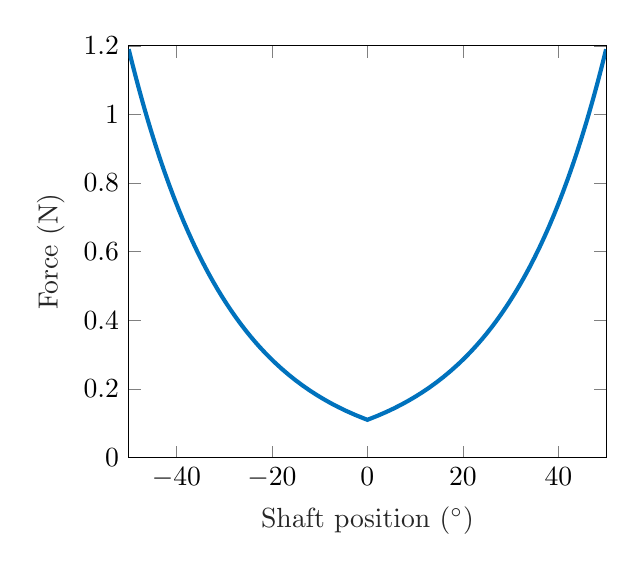
\begin{tikzpicture}

\begin{axis}[%
width=0.5\textwidth,
% width=4.472in,
% height=3.523in,
at={(0.75in,0.476in)},
scale only axis,
xmin=-50,
xmax=50,
xlabel style={font=\color{white!15!black}},
xlabel={Shaft position ($^\circ$)},
ymin=0,
ymax=1.2,
ylabel style={font=\color{white!15!black}},
ylabel={Force (N)},
axis background/.style={fill=white},
% title style={font=\bfseries},
% title={Logarithmic force - location relationship},
% xmajorgrids,
% ymajorgrids
]
\addplot [color=mycolor1, line width=1.5pt, forget plot]
  table[row sep=crcr]{%
-50	1.19\\
-49.5	1.16199810186362\\
-49	1.13465511658373\\
-48.5	1.10795553927742\\
-48	1.08188422990726\\
-47.5	1.05642640469615\\
-47	1.03156762774414\\
-46.5	1.00729380284255\\
-46	0.983591165480689\\
-45.5	0.96044627504066\\
-45	0.937846007175814\\
-44.5	0.915777546368624\\
-44	0.894228378663577\\
-43.5	0.87318628457114\\
-43	0.852639332138658\\
-42.5	0.83257587018435\\
-41.5	0.793854177351953\\
-40.5	0.756933364835092\\
-39.5	0.721729676742086\\
-38.5	0.688163252525818\\
-37.5	0.656157945817917\\
-36.5	0.625641151688548\\
-35.5	0.596543641940123\\
-34.5	0.568799408061217\\
-33.5	0.54234551148442\\
-32.5	0.517121940808416\\
-31.5	0.493071475660486\\
-30.5	0.470139556890473\\
-29.5	0.44827416280183\\
-28.5	0.427425691138978\\
-27.5	0.407546846563179\\
-26.5	0.388592533361745\\
-25.5	0.370519753147171\\
-24.5	0.3532875073141\\
-23.5	0.336856704032819\\
-22.5	0.321190069568381\\
-21.5	0.306252063724074\\
-20.5	0.292008799217513\\
-19.5	0.278427964806404\\
-18	0.259231769661341\\
-16.5	0.241359054750397\\
-15	0.224718572828124\\
-13.5	0.209225367683558\\
-12	0.194800340405337\\
-10.5	0.181369845550606\\
-9	0.16886531515604\\
-7.5	0.157222908671393\\
-6	0.146383187028384\\
-4.5	0.136290809180828\\
-2.5	0.123908300112632\\
-0.5	0.112650786425611\\
0	0.109999999999999\\
2	0.120992613055485\\
4	0.13308374921813\\
5.5	0.142938643253551\\
7	0.153523295332469\\
8.5	0.16489174427052\\
10	0.177102030474877\\
11.5	0.190216492263353\\
13	0.204302084126056\\
14.5	0.219430718554435\\
16	0.235679633182819\\
17.5	0.253131785116999\\
19	0.271876274462855\\
20	0.285137538166573\\
21	0.299045644318639\\
22	0.31363214384529\\
23	0.328930126627036\\
24	0.344974296563962\\
25	0.36180105030251\\
26	0.379448559802285\\
27	0.397956858930179\\
28	0.417367934278353\\
29	0.437725820411956\\
30	0.459076699762797\\
31	0.48146900739544\\
32	0.504953540883534\\
33	0.529583575545502\\
34	0.555414985301077\\
35	0.58250636942288\\
36	0.610919185470465\\
37	0.640717888708529\\
38	0.671970078325458\\
39	0.704746650783981\\
40	0.739121960651779\\
41	0.775173989276865\\
42	0.812984521690474\\
42.5	0.83257587018435\\
43	0.852639332138658\\
43.5	0.87318628457114\\
44	0.894228378663577\\
44.5	0.915777546368624\\
45	0.937846007175814\\
45.5	0.96044627504066\\
46	0.983591165480689\\
46.5	1.00729380284255\\
47	1.03156762774414\\
47.5	1.05642640469615\\
48	1.08188422990726\\
48.5	1.10795553927742\\
49	1.13465511658373\\
49.5	1.16199810186362\\
50	1.19\\
};
\end{axis}
\end{tikzpicture}%
  \caption{Logarithmic force location relationship}
  \label{fig:logarithmic_force_location}
\end{figure}

% section step_design (end)

\section{Limitations based on electronic system} % (fold)
\label{sec:limitations_based_on_electronic_system}

The forces and steps determined above are for an ideal system and are treated as a guide for choosing values for the real world application.

The RoboClaw motor controller, used to drive the motors, splits the voltage range (\SIrange{0}{24}{\volt}) into 128 steps (7 bit), resulting in a resolution of \SI{0.189}{\volt}.
Given the motor characterisation outlined in section X, it was found that the system has a current threshold of \SI{0.8}{\ampere} when the first logic level (\SI{0.189}{\volt}) was applied, as was shown in Figure~\ref{fig:motor_1}.

This means that, given the actual torque constant of $K_t$ determined in the motor characterisation in section~\ref{sec:motors}, the minimum torque applied by the motors is $0.8 K_t$. Thus, the minimum force on the surgeon's finger given the joystick length of \SI{11}{\centi\metre} is \SI{0.26}{\newton}.
Additionally, the current resolution (using the voltage resolution) is \SI{0.03}{\ampere}, which is 3.75\% of the \SI{0.8}{\ampere} minimum current, meaning increments of 10\% can be achieved.

To achieve the tested maximum force of \SI{1.19}{\newton}, the motors would need to apply \SI{143}{\milli\newton\metre} of torque. The following two sections will consider the thermal and stress analysis of our system to determine whether this torque can be applied.


% section limitations_based_on_electronic_system (end)

\section{Thermal Analysis} % (fold)
\label{sec:thermal_analysis}

To start with, the thermal characteristics of the motors were modelled at steady state for each current level, using the following assumptions:

\begin{itemize}
  \item Current is held constant long enough until the system is at thermal steady state
  \item Ambient temperature inside the casing is held constant at \SI{20}{\celsius}
  \item Thermal resistances given in the datasheet are correct
  \item At stall current, 80\% of the power flowing to the motors is converted into heat
\end{itemize}

The motors can be represented using the thermal circuit shown in Figure~\ref{fig:motor_thermals}.
To find the power flowing through the circuit at each current interval, the equation
\\
\begin{equation}
  P = I^2 R
\end{equation}

is used.
When the windings are at \SI{125}{\celsius}, their resistance is obtained using the temperature dependence equation,
\\
\begin{equation}
  R_{T=\SI{125}{\celsius}} = R_{T=\SI{20}{\celsius}} (1 + \alpha (\Delta T))
\end{equation}

where $\alpha$ is the temperature coefficient of resistance for copper (\SI{0.0004}{\per\kelvin}), giving $R_{T=\SI{125}{\celsius}} = \SI{8.1}{\ohm}$.

The temperature difference between the windings and ambient is then determined by equation~\ref{eq:temp_difference}, the temperature distribution is shown in Figure~\ref{fig:temp_windings}.
\\
\begin{equation}
  T_{difference} = Q R_{thermal} = 0.8 \times I^2 R_{electrical} \times R_{thermal}
  \label{eq:temp_difference}
\end{equation}

\begin{figure}
  % This file was created by matlab2tikz.
%
%The latest updates can be retrieved from
%  http://www.mathworks.com/matlabcentral/fileexchange/22022-matlab2tikz-matlab2tikz
%where you can also make suggestions and rate matlab2tikz.
%
\definecolor{mycolor1}{rgb}{0.00000,0.44700,0.74100}%
\centering

\begin{tikzpicture}

\begin{axis}[%
width=0.5\textwidth,
% width=4.472in,
% height=3.523in,
at={(0.75in,0.476in)},
scale only axis,
xmin=0,
xmax=3,
xlabel style={font=\color{white!15!black}},
xlabel={Current (A)},
ymin=0,
ymax=600,
ylabel style={font=\color{white!15!black}},
ylabel={$\text{T}_{\text{windings}}\text{ (}^\circ\text{C)}$},
axis background/.style={fill=white},
% title style={font=\bfseries},
% title={$\text{Steady State T}_{\text{windings}}\text{ for T}_{\text{casing}}\text{ = 20}^\circ\text{C based on current}$},
% xmajorgrids,
% ymajorgrids
]
\addplot [color=mycolor1, forget plot]
  table[row sep=crcr]{%
0	0\\
0.0235330109310325	0.0344254331334923\\
0.0470660218621788	0.137701732533856\\
0.0705990327932113	0.309828898201204\\
0.0941320437243576	0.550806930135536\\
0.11766505465539	0.86063582833674\\
0.141198065586536	1.23931559280493\\
0.164731076517569	1.6868462235401\\
0.188264087448715	2.20322772054215\\
0.211797098379748	2.78846008381117\\
0.23533010931078	3.44254331334707\\
0.258863120241926	4.16547740914996\\
0.282396131172959	4.95726237121983\\
0.305929142104105	5.81789819955657\\
0.329462153035138	6.74738489416029\\
0.352995163966284	7.74572245503089\\
0.376528174897317	8.81291088216858\\
0.400061185828463	9.94895017557303\\
0.423594196759495	11.1538403352446\\
0.447127207690642	12.427581361183\\
0.470660218621674	13.7701732533883\\
0.494193229552707	15.1816160118607\\
0.517726240483853	16.6619096365998\\
0.541259251414886	18.2110541276061\\
0.564792262346032	19.8290494848792\\
0.588325273277064	21.5158957084193\\
0.611858284208211	23.2715927982263\\
0.635391295139243	25.0961407543002\\
0.682457317001422	28.951789265249\\
0.729523338863601	33.0828412412654\\
0.776589360725779	37.4892966823497\\
0.823655382587958	42.1711555885017\\
0.870721404450137	47.1284179597216\\
0.917787426312316	52.3610837960091\\
0.964853448174381	57.8691530973645\\
1.01191947003656	63.6526258637875\\
1.05898549189874	69.7115020952784\\
1.10605151376092	76.045781791837\\
1.1531175356231	82.6554649534635\\
1.20018355748527	89.5405515801576\\
1.24724957934745	96.7010416719196\\
1.29431560120963	104.136935228749\\
1.34138162307181	111.848232250647\\
1.38844764493388	119.834932737612\\
1.43551366679606	128.097036689645\\
1.48257968865823	136.634544106746\\
1.52964571052041	145.447454988914\\
1.57671173238259	154.535769336151\\
1.62377775424477	163.899487148455\\
1.67084377610695	173.538608425827\\
1.71790979796913	183.453133168266\\
1.76497581983131	193.643061375774\\
1.81204184169349	204.108393048349\\
1.85910786355555	214.849128185992\\
1.90617388541773	225.865266788702\\
1.97677291821105	242.90585618977\\
2.04737195100427	260.566103387241\\
2.11797098379748	278.846008381114\\
2.1885700165908	297.745571171389\\
2.25916904938401	317.264791758067\\
2.32976808217722	337.403670141148\\
2.40036711497055	358.162206320631\\
2.47096614776376	379.540400296516\\
2.54156518055697	401.538252068804\\
2.6121642133503	424.155761637494\\
2.68276324614351	447.392929002587\\
2.75336227893683	471.249754164082\\
2.82396131173005	495.72623712198\\
2.89456034452326	520.82237787628\\
2.96515937731658	546.538176426983\\
};
\end{axis}
\end{tikzpicture}%
  \caption{Steady state $T_{windings}$ for $T_{casing} = \SI{20}{\degree}$ based on current}
  \label{fig:temp_windings}
\end{figure}

The maximum temperature which the windings can sustain is \SI{125}{\degree}, meaning only torques up to \SI{45.5}{\milli\newton\metre} can be applied continuously, as outlined in the datasheet.
As this would only give us a small range of \SIrange{28.8}{45}{\milli\newton\metre}, we needed to determine how long each torque step over \SI{45.5}{\milli\newton\metre} could be applied before the windings reach \SI{125}{\degree}.

To do this, the worst case scenario was analysed based on the following assumptions:

\begin{itemize}
  \item All power ($I^2R_{electrical}$) is used to increase the temperature of the windings
  \item The temperature of the windings rises at a constant rate
  \item The resistance ($R_{electrical}$) is taken as the mean resistance, i.e. $R_{electrical,\SI{75}{\celsius}}$
  \item Mass of the windings is \SI{50}{\gram}
\end{itemize}

Then, the time taken was calculated using equation~\ref{eq:heating_time}, giving the distribution shown in Figure~\ref{fig:overheating_times}.
\\
\begin{equation}
  t = \frac{m c_p \Delta T}{I^2 R_{electrical, \SI{72.5}{\celsius}}}
  \label{eq:heating_time}
\end{equation}

\begin{figure}
  % This file was created by matlab2tikz.
%
%The latest updates can be retrieved from
%  http://www.mathworks.com/matlabcentral/fileexchange/22022-matlab2tikz-matlab2tikz
%where you can also make suggestions and rate matlab2tikz.
%
\definecolor{mycolor1}{rgb}{0.00000,0.44700,0.74100}%
\centering
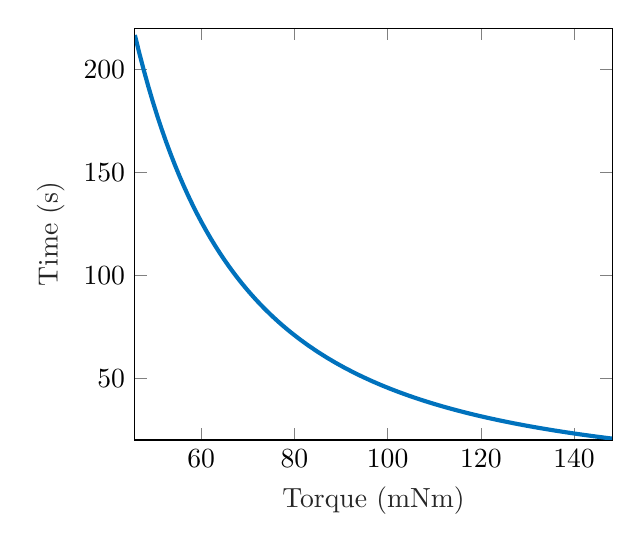
\begin{tikzpicture}

\begin{axis}[%
width=0.5\textwidth,
% width=4.472in,
% height=3.523in,
at={(0.75in,0.476in)},
scale only axis,
xmin=45.76,
xmax=148.192,
xlabel style={font=\color{white!15!black}},
xlabel={Torque (mNm)},
ymin=20,
ymax=220,
ylabel style={font=\color{white!15!black}},
ylabel={Time (s)},
axis background/.style={fill=white},
% title style={font=\bfseries},
% title={$\text{Time torque can be applied before T}_{\text{windings}}\text{=125}^\circ\text{C}$}
]
\addplot [color=mycolor1, line width=1.5pt, forget plot]
  table[row sep=crcr]{%
45.76	216.667738615899\\
46.717308411215	207.879017576417\\
47.6746168224299	199.614396388717\\
48.6319252336449	191.83301684817\\
49.5892336448598	184.497926086804\\
50.5465420560748	177.575637049549\\
51.5038504672897	171.035745616566\\
52.4611588785047	164.850596179228\\
53.4184672897196	158.994988786501\\
54.3757757009346	153.445922059341\\
55.3330841121495	148.182366966195\\
56.2903925233645	143.185067297208\\
57.2477009345795	138.436363295865\\
58.2050093457944	133.92003542655\\
59.1623177570094	129.621165692925\\
60.1196261682243	125.526014289477\\
61.0769345794393	121.621909678926\\
62.0342429906542	117.897150450992\\
62.9915514018692	114.340917541211\\
63.9488598130841	110.943195578534\\
64.9061682242991	107.694702292625\\
65.863476635514	104.586825050636\\
66.820785046729	101.61156371225\\
67.778093457944	98.7614790942068\\
68.7354018691589	96.0296464237145\\
69.6927102803739	93.4096132363436\\
70.6500186915888	90.8953612399318\\
71.6073271028038	88.481271723208\\
72.5646355140187	86.1620941375275\\
73.5219439252337	83.9329175233695\\
74.4792523364486	81.7891444909861\\
75.4365607476636	79.7264674975661\\
76.3938691588785	77.7408471921507\\
77.3511775700935	75.8284926248582\\
78.3084859813084	73.98584313922\\
79.2657943925234	72.2095517860033\\
81.1804112149533	68.8436342096961\\
83.0950280373832	65.7076907884335\\
85.0096448598131	62.7812384363757\\
86.924261682243	60.0460247636405\\
88.8388785046729	57.4857427824309\\
90.7534953271028	55.0857872919944\\
92.6681121495327	52.8330461261715\\
94.5827289719626	50.7157206762131\\
96.4973457943925	48.7231710891233\\
98.4119626168224	46.8457823391547\\
100.326579439252	45.0748480167701\\
102.241196261682	43.4024692061446\\
104.155813084112	41.8214662531165\\
106.070429906542	40.3253015792899\\
107.985046728972	38.9080119896234\\
109.899663551402	37.5641491621207\\
111.814280373832	36.2887272085666\\
113.728897196262	35.0771763621447\\
115.643514018692	33.9253019872727\\
117.558130841122	32.8292482239533\\
119.472747663551	31.7854656773205\\
121.387364485981	30.7906826460408\\
124.259289719626	29.3838398640721\\
127.131214953271	28.0712587444694\\
130.003140186916	26.844702586973\\
132.875065420561	25.696815090787\\
135.746990654206	24.6210097977903\\
138.61891588785	23.6113754002697\\
141.490841121495	22.6625943638046\\
144.36276635514	21.7698727677248\\
147.234691588785	20.9288796301169\\
148.192	20.6593552429105\\
};
\end{axis}
\end{tikzpicture}%
  \caption{Time torque can be applied before $T_{windings} = \SI{125}{\celsius}$}
  \label{fig:overheating_times}
\end{figure}

Where $c_p$ is the heat capacity of copper.

Using the times obtained above, we find that the motors can be at maximum torque for 20 seconds before the windings reach their maximum temperature, a very unlikely situation given their application. During use, the surgeon is expected to spend most of the time inside the "go-zone" where the motors are switched off.
Therefore, it is fine to use the motors up to our desired maximum torque of \SI{143}{\milli\newton\metre}.


% section thermal_analysis (end)

\section{Stress Analysis} % (fold)
\label{sec:stress_analysis}

% section stress_analysis (end)

\section{Conclusion} % (fold)
\label{sec:conclusion}

% section conclusion (end)